\section{Lista 4: Método dos Mínimos Quadrados} % <-----------------------------------------------------------------------------

\subsection{Algoritmo RLS} % <-----------------------------------------------------------------------------
As tabelas~\ref{tab:fixcoef} e \ref{tab:freecoef} apresentas as 10 primeiras iterações dos coeficientes de filtro, para caso $w_0$ seja fixo igual a um ou possa atualizar livremente. É possível observar que a oscilação fica cada menor ao se aproximar da 10ª iteração.

\begin{table}[!htp]
    \centering
    \begin{tabular}{ l l l l }
        \hline
        Iterations & $w_{0}$ & $w_{1}$ & $w_{2}$ \\ 
        \hline 
        1 & 1 & 0 & 0 \\ \hline
        2 & - & -0.0161 & -0.0130 \\ \hline
        3 & - & -0.0168 & -0.0472 \\ \hline
        4 & - & 0.0048 & -0.0518 \\ \hline
        5 & - & 0.0320 & -0.0831 \\ \hline
        6 & - & 0.0504 & -0.0561 \\ \hline
        7 & - & -0.0231 & 0.0466 \\ \hline
        8 & - & 0.0630 & 0.1069 \\ \hline
        9 & - & 0.0568 & 0.1192 \\ \hline
        10 & - & 0.0796 & 0.1457 \\ \hline
    \end{tabular}
    \caption{Atualização do filtro com o $w_0$ fixo igual a um.}
    \label{tab:fixcoef}
\end{table}

\begin{table}[!htp]
    \centering
    \begin{tabular}{l l l l}
        \hline
        Iterations & $w_{0}$ & $w_{1}$ & $w_{2}$ \\ 
        \hline \hline
        1 & 1 & 0 & 0 \\ \hline
        2 & 0.9860 & -0.0161 & -0.0130 \\ \hline
        3 & 0.9611 & -0.0167 & -0.0435 \\ \hline
        4 & 0.9687 & 0.0134 & -0.0499 \\ \hline
        5 & 0.9322 & 0.0369 & -0.0769 \\ \hline
        6 & 0.9053 & 0.0609 & -0.0419 \\ \hline
        7 & 0.8471 & 0.0034 & 0.0384 \\ \hline
        8 & 0.7149 & 0.0642 & 0.0809 \\ \hline
        9 & 0.7264 & 0.0767 & 0.0558 \\ \hline
        10 & 0.7125 & 0.0843 & 0.0646 \\ \hline
    \end{tabular}
    \caption{Atualização do filtro com o $w_0$ livre para atualizar.}
    \label{tab:freecoef}
\end{table}

A título de comparação, foi implementado ambos os casos de atualização do coeficientes $w_0$. A Figura~\ref{fig:hw4p1} mostra os sinais obtidos com ambos os vetores de filtro, que se aproximam consideravelmente do sinal original, senoidal entre $(-3\pi,3\pi)$.

Na inicialização do filtro, ambos distam igualmente do sinal desejado, porém ao passo que mais amostras são utilizadas no processo de adaptação, ambos se aproximam do sinal alvo. Apresentando maiores oscilações justamente nos pontos inflexão, dado a variação mais abrupta.

É possível observar também que o algoritmo com livre adaptação para $w_0$ apresenta desempenho melhor que o proposto, dado que existe um coeficiente a mais para garantir que a adaptação será mais adequada que ao manter um valor fixo e atualizar apenas dois coeficientes.

\clearpage

\begin{figure}[!htp]
    \centering
    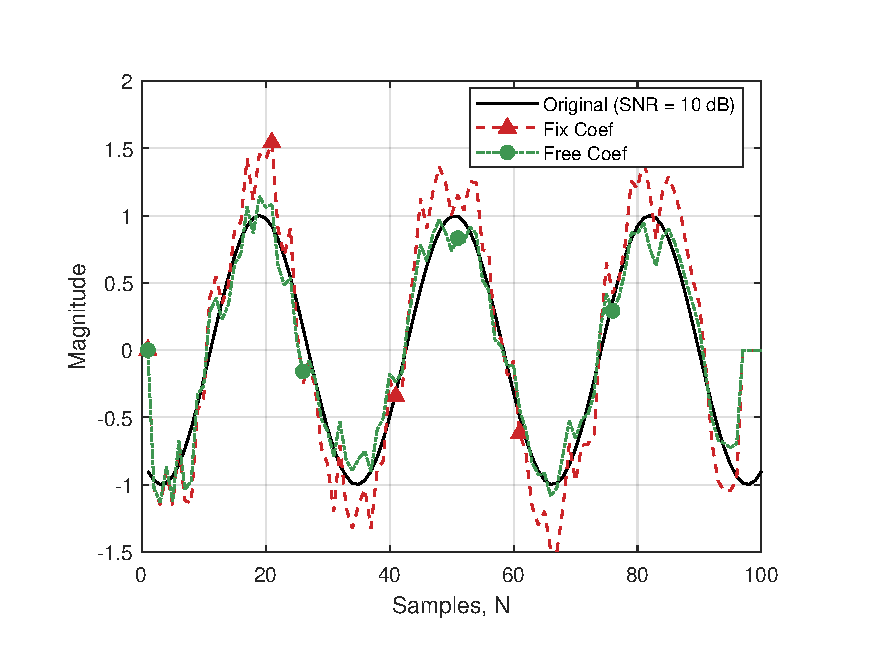
\includegraphics[width=1.0\textwidth]{C:/Users/lucasabdalah-dell/Documents/GitHub/Courses-HWs/Master/TIP7188-FILTRAGEM_ADAPTATIVA/homework/code/figures/hw4p1.pdf}
    \caption{Primeiro coeficiente livre para adaptação com $\text{Amostras} = 100$, $M = 2$, $\lambda = 0.98$}
    \label{fig:hw4p1}
\end{figure}


\subsection{Erro de Estimação a Priori} % <-----------------------------------------------------------------------------

De partida, é necessário relacionar o error $e(n)$ e o erro a priori $\epsilon(n)$. Utilizando a expressão recursiva de $w(n)$ no instante $n$, de modo que: $\mathbf{w}(n) = \mathbf{w}(n-1) + \epsilon(n) \mathbf{S}_{D}(n) \mathbf{x}(n)$.
\begin{align*}
    e(n) &= d(n) - \mathbf{w}^{\text{H}}(n) \mathbf{x}(n) \\
    &= d(n) - \mathbf{x}^{\text{H}}(n) \mathbf{w}(n) \\
    &= d(n) - \mathbf{x}^{\text{H}}(n) \left[\mathbf{w}(n-1) + \epsilon(n) \mathbf{S}_{D}(n) \mathbf{x}(n)\right] \\
    &= d(n) - \mathbf{x}^{\text{H}}(n) \mathbf{w}(n-1) - \mathbf{x}^{\text{H}}(n) \epsilon(n) \mathbf{S}_{D}(n) \mathbf{x}(n) \\
\end{align*}

Dado que $\epsilon(n) = d(n) - \mathbf{x}^{\text{H}}(n) \mathbf{w}(n-1)$, obtém-se:
\begin{align*}
    e(n) &= \epsilon(n) - \epsilon(n) \mathbf{x}^{\text{H}}(n) \mathbf{S}_{D}(n) \mathbf{x}(n) \\
    &= \epsilon(n) - \epsilon(n) \mathbf{x}^{\text{H}}(n) \mathbf{S}_{D}(n) \mathbf{x}(n) \\
\end{align*}

Conjugando o elemento de erro $e(n)$ e no lado direito da expressão, pdemos introduzir o termo que representa a chamada distância de Mahalanobis $M_D$, logo temos:
\begin{align*}
    e^{*}(n) &= \epsilon^{*}(n) - \epsilon^{*}(n) \mathbf{x}^{\text{H}}(n) \mathbf{S}_{D}(n) \mathbf{x}(n) \\
    &= \epsilon^{*}(n) - \epsilon^{*}(n) M_D \\
    &= \epsilon^{*}(n) (1 - M_D)
\end{align*}

Multiplicando a expressão pelo erro $e(n)$ à esquerda, é possível avaliar a questão numérica:
\begin{align*}
    \epsilon(n) e^{*}(n) &= \epsilon(n) \epsilon^{*}(n) \left(1 - M_D \right).
\end{align*}

Podemos observar que 
\begin{enumerate}
    \item Dado que $M_D$ é distância, é sempre real e positiva, logo $\left(1 - M_D \right)$ é sempre real;
    \item Enquanto $\epsilon(n) \epsilon^{*}(n)$ é uma norma dada por $||\epsilon(n)||^{2} = \epsilon(n), \epsilon^{*}(n)$, sempre posivitiva e real.
\end{enumerate}

Isto permite concluir que o produto do erro pelo seu conjugado será sempre real.


\subsection{Preditor Adaptativo} % <-----------------------------------------------------------------------------

As Figuras~\ref{fig:hw4p3-fig1}, \ref{fig:hw4p3-fig2}, mostram o comportamento do RLS para um cenário de SNR $=$ 3 dB, e a medida que $\lambda$ aumenta uma casa decimal com 9, o erro médio diminui, se aproxima de um valor estável, mas os coeficientes do filtro não convergem.

\begin{figure}[!htp]
    \centering
    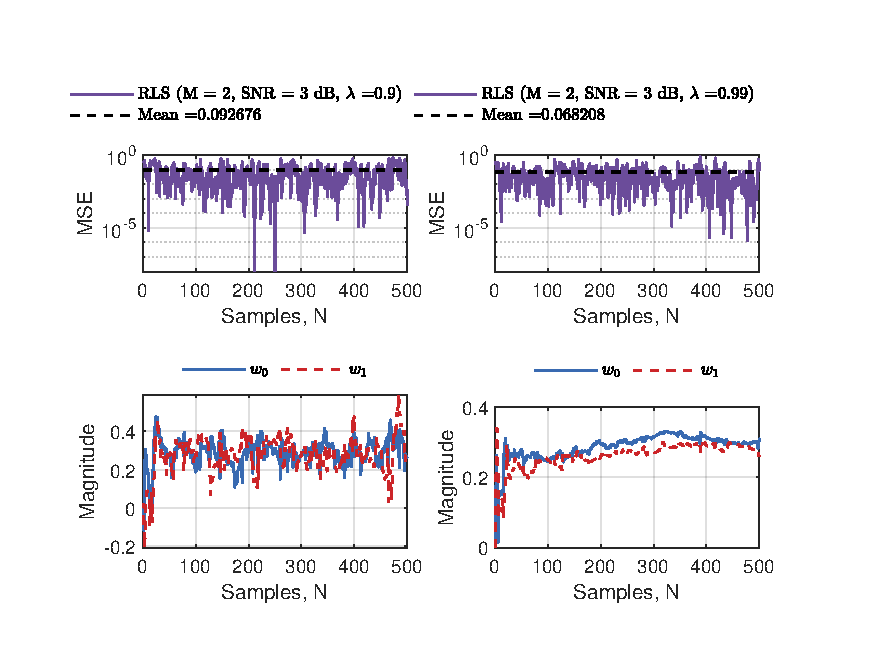
\includegraphics[width=0.8\textwidth]{C:/Users/lucasabdalah-dell/Documents/GitHub/Courses-HWs/Master/TIP7188-FILTRAGEM_ADAPTATIVA/homework/code/figures/hw4p3-fig1.pdf}
    \caption{RLS com 500 amostras, $M=2$, SNR = 3dB, variando $\lambda$.}
    \label{fig:hw4p3-fig1}
\end{figure}

\clearpage

\begin{figure}[!htp]
    \centering
    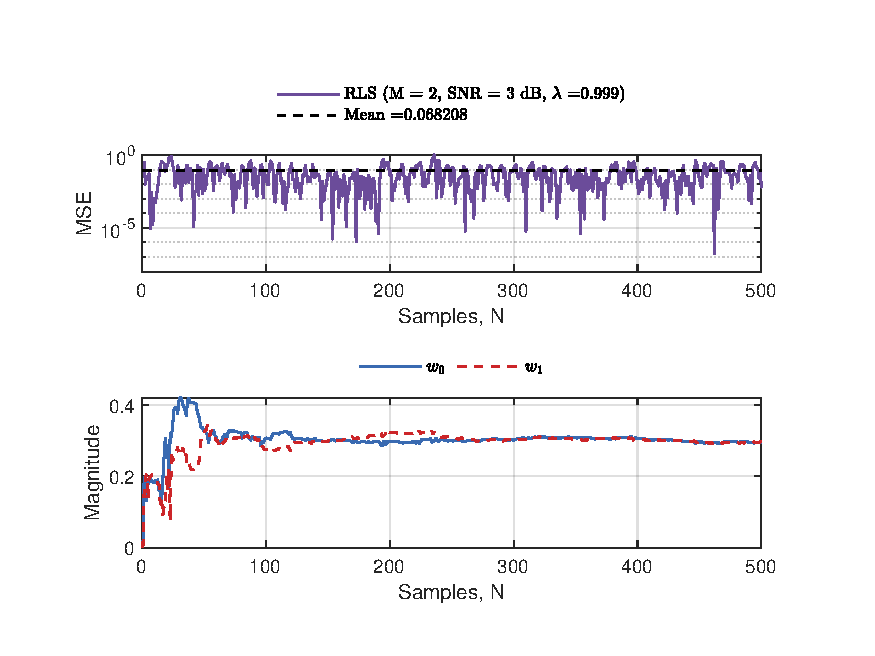
\includegraphics[width=0.8\textwidth]{C:/Users/lucasabdalah-dell/Documents/GitHub/Courses-HWs/Master/TIP7188-FILTRAGEM_ADAPTATIVA/homework/code/figures/hw4p3-fig2.pdf}
    \caption{RLS com 500 amostras, $M=2$, SNR = 3dB, com $\lambda = 0.999$.}
    \label{fig:hw4p3-fig2}
\end{figure}

As Figuras~\ref{fig:hw4p3-fig3}, \ref{fig:hw4p3-fig4},mostram o comportamento do RLS para um cenário de SNR $\rightarrow \infty$ dB. Para $\lambda =0.9$, o algoritmo diverge abruptamente. Entretanto, para $\lambda = \{0.99, 0.999\}$ o erro médio é muito abaixo dos outros cenários, enquanto os coeficientes do filtro convergem para o valor estável de pesos.

A análise análoga é feita para as Figuras~\ref{fig:hw4p3-fig5}-\ref{fig:hw4p3-fig8}, sendo que desta vez a ordem do filtro é de $M=3$.

\begin{figure}[!htp]
    \centering
    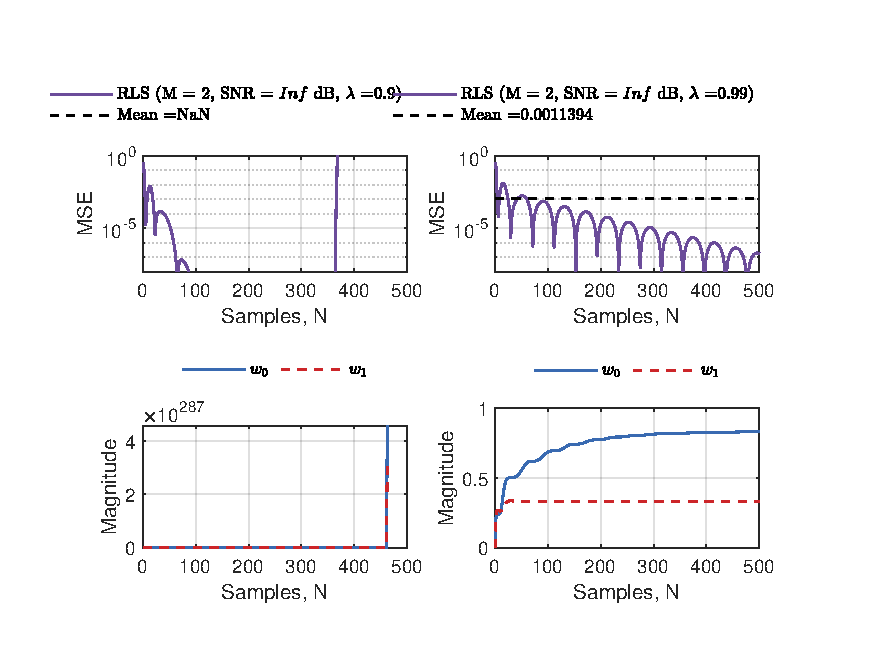
\includegraphics[width=0.8\textwidth]{C:/Users/lucasabdalah-dell/Documents/GitHub/Courses-HWs/Master/TIP7188-FILTRAGEM_ADAPTATIVA/homework/code/figures/hw4p3-fig3.pdf}
    \caption{RLS com 500 amostras, $M=3$, SNR = $\infty$dB, variando $\lambda$.}
    \label{fig:hw4p3-fig3}
\end{figure}


\begin{figure}[!htp]
    \centering
    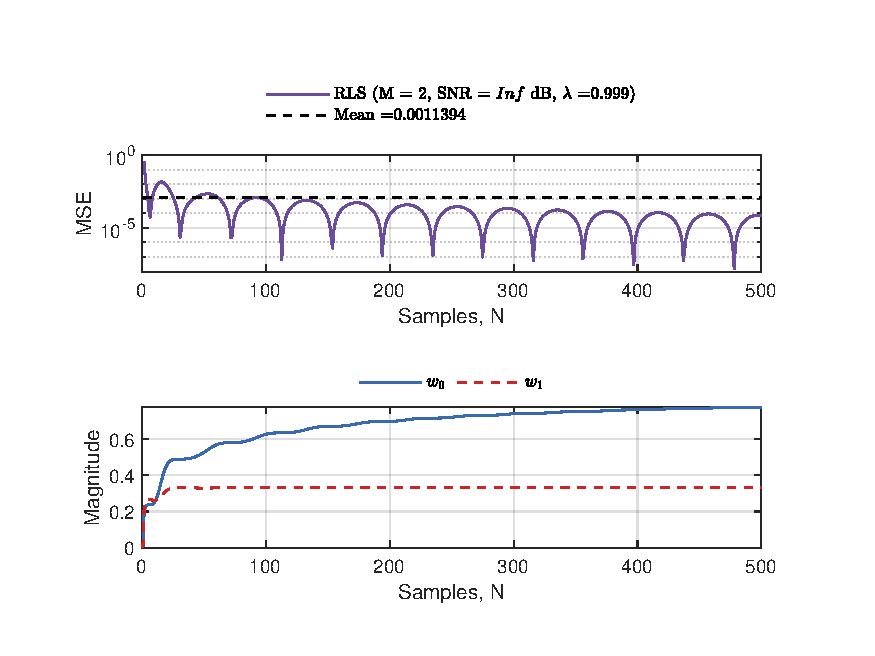
\includegraphics[width=0.8\textwidth]{C:/Users/lucasabdalah-dell/Documents/GitHub/Courses-HWs/Master/TIP7188-FILTRAGEM_ADAPTATIVA/homework/code/figures/hw4p3-fig4.pdf}
    \caption{RLS com 500 amostras, $M=2$, SNR = $\infty$dB, $\lambda = 0.999$.}
    \label{fig:hw4p3-fig4}
\end{figure}

\begin{figure}[!htp]
    \centering
    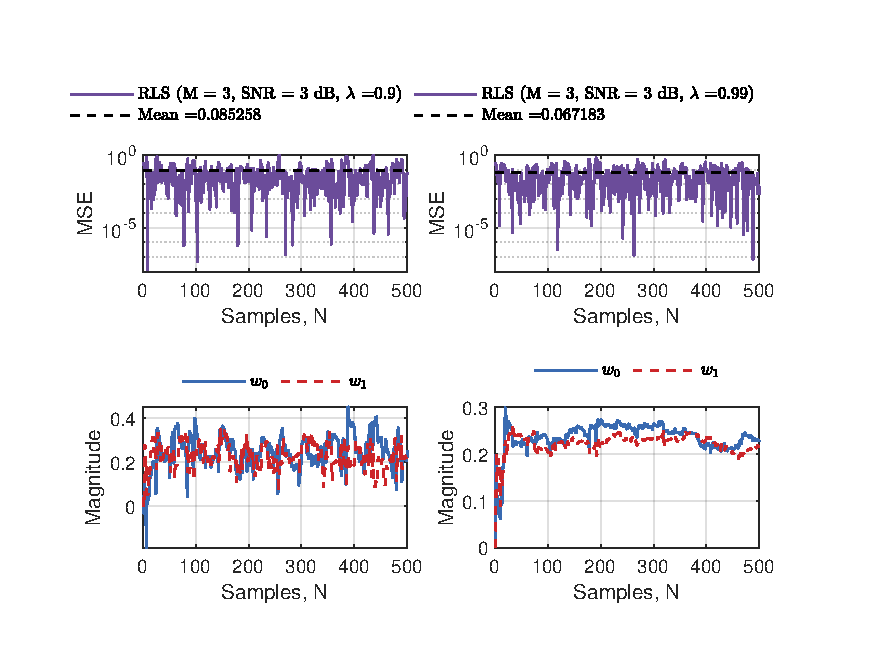
\includegraphics[width=0.8\textwidth]{C:/Users/lucasabdalah-dell/Documents/GitHub/Courses-HWs/Master/TIP7188-FILTRAGEM_ADAPTATIVA/homework/code/figures/hw4p3-fig5.pdf}
    \caption{RLS com 500 amostras, $M=3$, SNR = 3dB, variando $\lambda$.}
    \label{fig:hw4p3-fig5}
\end{figure}

\begin{figure}[!htp]
    \centering
    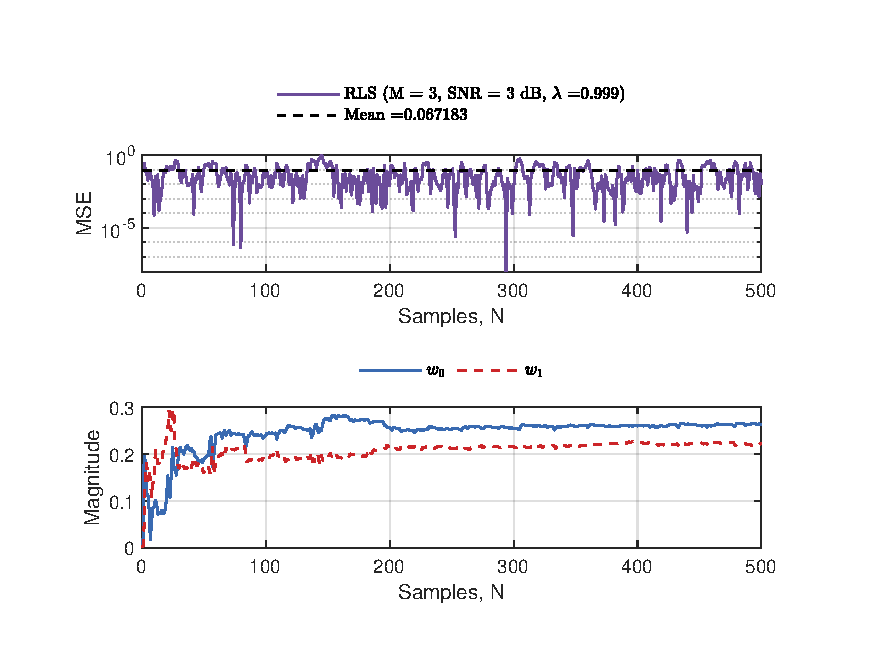
\includegraphics[width=0.8\textwidth]{C:/Users/lucasabdalah-dell/Documents/GitHub/Courses-HWs/Master/TIP7188-FILTRAGEM_ADAPTATIVA/homework/code/figures/hw4p3-fig6.pdf}
    \caption{RLS com 500 amostras, $M=3$, SNR = 3dB, com $\lambda = 0.999$.}
    \label{fig:hw4p3-fig6}
\end{figure}

\begin{figure}[!htp]
    \centering
    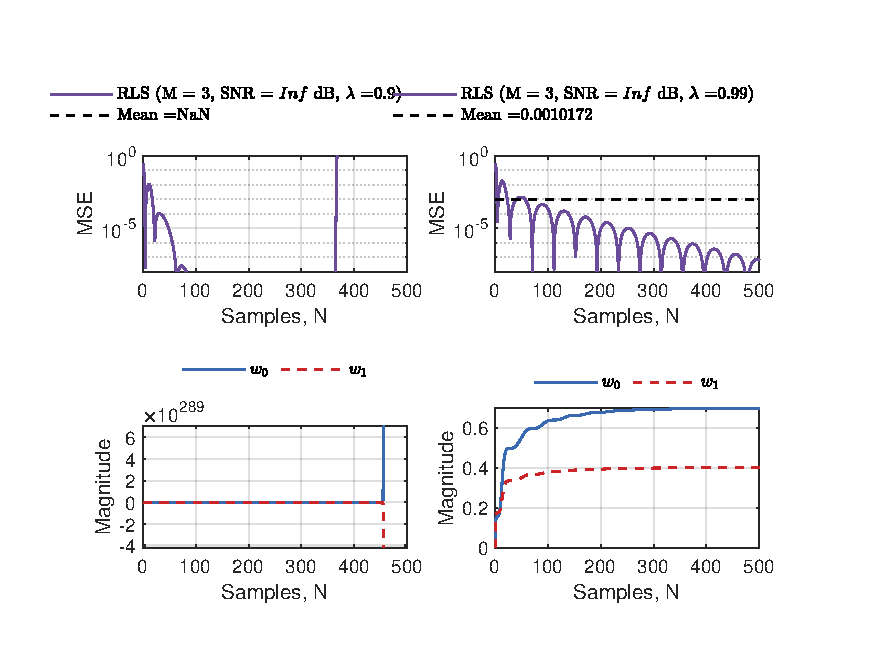
\includegraphics[width=0.8\textwidth]{C:/Users/lucasabdalah-dell/Documents/GitHub/Courses-HWs/Master/TIP7188-FILTRAGEM_ADAPTATIVA/homework/code/figures/hw4p3-fig7.pdf}
    \caption{RLS com 500 amostras, $M=3$, SNR = $\infty$dB, variando $\lambda$.}
    \label{fig:hw4p3-fig7}
\end{figure}

\begin{figure}[!htp]
    \centering
    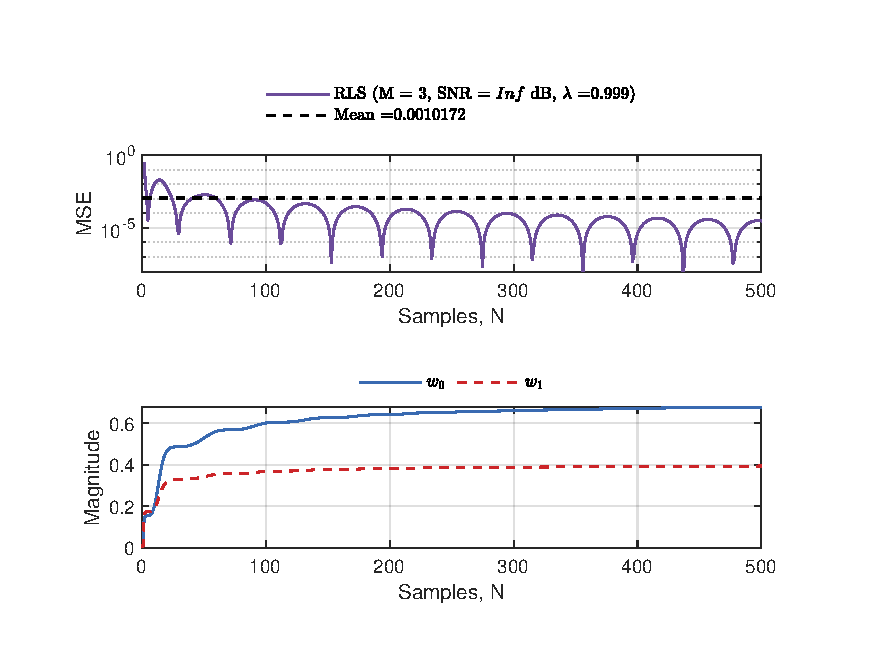
\includegraphics[width=0.8\textwidth]{C:/Users/lucasabdalah-dell/Documents/GitHub/Courses-HWs/Master/TIP7188-FILTRAGEM_ADAPTATIVA/homework/code/figures/hw4p3-fig8.pdf}
    \caption{RLS com 500 amostras, $M=3$, SNR = $\infty$dB, $\lambda = 0.999$.}
    \label{fig:hw4p3-fig8}
\end{figure}

\clearpage


\subsection{Equalização de Canais} % <-----------------------------------------------------------------------------
% \todo[inline, color=red!30]{Finalizar}
% \begin{enumerate}
    
%     \item Calcule a adaptação do algoritmo usando o RLS e mostre a evolução temporal dos coeficientes.

%         \textcolor{red}{Solução:}

%         A evolução temporal dos coeficientes do filtro pode ser encontrada na Figura \ref{fig:rls_coefficient}.  
%         Aqui é possível verificar a convergência e estabilização dos coeficientes do filtro partindo do zero a medida que o número 
%         de iterações cresce. Existem algumas oscilações ao final do processo, mas nada considerável. Caso o fator de esquecimento fosse
%         aumentado possivelmente haveriam oscilações com maiores magnitudes nos coeficientes de filtro. 

%     \item Obtenha as trajetórias sobre as curvas de nível, tendo condições iniciais nulas para os
%     coeficientes do equalizador. Verifique qual a melhor inicialização do algoritmo RLS. Compare
%     com os algoritmos LMS, LMS-Normalizado e Gauss-Newton.

%         \textcolor{red}{Solução:}

%         As trajetórias dos algoritmos Newton, Gradiente, LMS e NLMS estão disponíveis nas Figuras \ref{fig:newton_contour}, \ref{fig:gradient_contour}, 
%         \ref{fig:lms_contour} e \ref{fig:nlms_contour}. Na Figura \ref{fig:rls_contour} é apresentado o traçado da trajetória de convergência para o RLS.
%         É possível verificar que o RLS apresenta um comportamento de convergência na superfície MSE mais próximo do algoritmo LMS. Existem alguns outliers durante 
%         o processo de filtragem, mas de modo geral o filtro tende à solução ótima de uma forma mais organizada e estável do que o NLMS.

%     \item Obtenha também a evolução do erro quadrático médio para cada um dos algoritmos anteriores.

%         \textcolor{red}{Solução:} 

%         As evolução do erro quadrático médio para os algoritmos Newton, Gradiente, LMS e NLMS já foram abordadas na seção 
%         anterior e podem ser revisitadas nas Figuras \ref{fig:newton_mse}, \ref{fig:gradient_mse}, \ref{fig:lms_mse} e \ref{fig:nlms_mse}.
%         adicionalmente, o traçado da evolução do MSE para o método RLS está presente na Figura \ref{fig:rls_mse}. Nessa figura podemos verificar
%         que o RLS apresenta uma latência de convergência menor que o LMS e NLMS, mas ao final do processo aparentemente o grau de estabilidade da
%         solução dos coeficientes de filtro parece ser menor do que quando comparamos com os quatro algoritmos de filtragem mencionados anteriormente.


% \begin{figure}[!htp]
%     \centering
%     % \includegraphics[width=0.75\textwidth]{figs/rls_coefficients.png}
%     \includegraphics[width=0.5\textwidth]{example-image}
%     \caption{Convergência dos coeficientes para o RLS. $\text{Amostras} = 5000$, $M = 2$, $\lambda = 0.99$}
%     \label{fig:rls_coefficient}
% \end{figure}

% \begin{figure}[!htp]
%     \centering
%     % \includegraphics[width=0.75\textwidth]{figs/rls_contour.png}
%     \includegraphics[width=0.5\textwidth]{example-image}
%     \caption{Caminho de convergência na superficie MSE para o RLS. $\text{Amostras} = 5000$, $M = 2$, $\lambda = 0.99$}
%     \label{fig:rls_contour}
% \end{figure}

% \begin{figure}[!htp]
%     \centering
%     % \includegraphics[width=0.75\textwidth]{figs/rls_mse.png}
%     \includegraphics[width=0.5\textwidth]{example-image}
%     \caption{Comportamento da evolução do MSE para o RLS. $\text{Amostras} = 5000$, $M = 2$, $\lambda = 0.99$}
%     \label{fig:rls_mse}
% \end{figure}

% \end{enumerate}


\subsection{Equalização Adaptativa} % <-----------------------------------------------------------------------------
% \todo[inline, color=red!30]{Finalizar}

% Assim como na questão da lista anterior foi considerado novamente que o filtro é de ordem $M = 15$.
% Os resultados podem ser encontrados nas Figuras \ref{fig:L4Q5_a1}, \ref{fig:L4Q5_a2}, \ref{fig:L4Q5_a3} e \ref{fig:L4Q5_a4}.
% Inicialmente é possível confirmar uma evidente vantagem na velocidade de convergência do RLS quando o comparamos com o algoritmo LMS.
% Independentemente do fator de esquecimento considerado todos apresentam uma vantagem considerável sobre o LMS quando se observa tanto a 
% latência quanto o desempenho da evolução do MSE. Desse modo, o RLS tem menor latência e melhor desempenho MSE quando comparamos com o LMS.

% Já quando voltamos nossa análise para o impacto do fator de esquecimento é possível verificar uma interessante característica do 
% RLS. O fator de esquecimento atua de forma semelhante ao passo de aprendizado nos algoritmos LMS e NLMS, mas num sentido um  pouco diferente. Desse modo, quanto
% maior o seu valor mais flexível torna-se o filtro para adaptar-se a novos estímulos. Assim, nas Figuras \ref{fig:L4Q5_a2} e \ref{fig:L4Q5_a3}, onde o 
% fator de esquecimento é definido respectivamente por $\lambda = 0.9$ e $\lambda = 0.99$, é possível ver que o MSE apresenta oscilações de 
% elevadas magnitudades mesmo após a convergência pois estamos restringindo a flexibilidade do RLS. Já na Figura \ref{fig:L4Q5_a4} onde temos um fator de esquecimento 
% definido por $\lambda = 0.999$ temos oscilações de magnitudades consideravelmente menores quando comparamos com os dois casos anteriores. Já com relação ao valor de convergência
% MSE não é possível notar grandes diferenças entre os casos considerados, visto que todos oscilam em torno de um valor aproximadamente igual.

% Por fim, nas Figuras \ref{fig:L4Q5_a5} e \ref{fig:L4Q5_a6} são traçados os gráficos da evolução temporal e da resposta em frequência para
% o cenário proposto, respectivamente. Na primeira figura vemos a adaptação do algoritmo RLS a medida que o número de iterações progride e, apesar do
% equalizador desconhecer o sinal verdadeiro, existe uma aparente melhora de desempenho a medida que o filtro progride. Já na figura seguinte são comparados
% diretamente as repostas em frequência dos filtros LMS e RLS em relação ao sistema desconhecido com $\mu = 0.001$ e $\lambda = 0.999$, respectivamente.
% A partir de tal resultado podemos verificar que o filtro RLS consegue adaptar-se mais facilmente ao sistema desconhecido enquanto o filtro LMS apresenta
% intensas variações que possivelmente prejudicariam o processo de filtragem.


% \begin{figure}[!htp]
%     \centering
%     % \includegraphics[width=0.75\textwidth]{figs/L4Q5_lms.png}
%     \includegraphics[width=0.5\textwidth]{example-image}
%     \caption{Comportamento da evolução do MSE para o LMS. $\text{Amostras} = 500$, $M = 15$, $\mu = 0.001$}
%     \label{fig:L4Q5_a1}
% \end{figure}

% \begin{figure}[!htp]
%     \centering
%     % \includegraphics[width=0.75\textwidth]{figs/L4Q5_rls_9.png}
%     \includegraphics[width=0.5\textwidth]{example-image}
%     \caption{Comportamento da evolução do MSE para o RLS. $\text{Amostras} = 500$, $M = 15$, $\lambda = 0.9$}
%     \label{fig:L4Q5_a2}
% \end{figure}

% \begin{figure}[!htp]
%     \centering
%     % \includegraphics[width=0.75\textwidth]{figs/L4Q5_rls_99.png}
%     \includegraphics[width=0.5\textwidth]{example-image}
%     \caption{Comportamento da evolução do MSE para o RLS. $\text{Amostras} = 500$, $M = 15$, $\lambda = 0.99$}
%     \label{fig:L4Q5_a3}
% \end{figure}

% \begin{figure}[!htp]
%     \centering
%     % \includegraphics[width=0.75\textwidth]{figs/L4Q5_rls_999.png}
%     \includegraphics[width=0.5\textwidth]{example-image}
%     \caption{Comportamento da evolução do MSE para o RLS. $\text{Amostras} = 500$, $M = 15$, $\lambda = 0.999$}
%     \label{fig:L4Q5_a4}
% \end{figure}

% \begin{figure}[!htp]
%     \centering
%     % \includegraphics[width=0.75\textwidth]{figs/L4Q5_rls_t.png}
%     \includegraphics[width=0.5\textwidth]{example-image}
%     \caption{Evolução temporal para o RLS. $\text{Amostras} = 500$, $M = 15$, $\lambda = 0.999$}
%     \label{fig:L4Q5_a5}
% \end{figure}

% \begin{figure}[!htp]
%     \centering
%     % \includegraphics[width=0.75\textwidth]{figs/L4Q5_filter_response.png}
%     \includegraphics[width=0.5\textwidth]{example-image}
%     \caption{Comparativo da resposta em frequência para LMS e RLS. $\text{Amostras} = 500$, $M = 15$, $\lambda = 0.999$}
%     \label{fig:L4Q5_a6}
% \end{figure}

